\begin{twierdzenie}(Lemat Newmana)\label{thm:newman_lemma}
Niech \(\to\) bedzie relacją binarną mającą własność SN. Jeśli \(\to\) ma własność WCR, to \(\to\) ma własność CR.
\end{twierdzenie}

\begin{dowod}


Niech \(\to\) będzie relacją binarną na \(A\) o własności SN i WCR. Ponieważ \(\to\) jest SN, to każdy \(a\) jest normalizowalny. Powiemy, że \(a\) jest \emph{wieloznaczny}, jeśli \(a\) redukuje się do dwóch różnych postaci normalnych.

Rozważmy następujące przypadki:

\begin{minipage}{.75\textwidth}
\begin{enumerate}[label={\roman*)}, ref={\roman*)}]
  \setlength\itemsep{0em}
  \item Niech \(a\in A\). Jeśli \(a\) nie jest wieloznaczny, to teza zachodzi.
  \item 
      Przypuśćmy, że \(a\) jest wieloznaczny. wówczas istnieje inny \(a'\in A\), który też jest wieloznaczny oraz \(a\to a'\). Istotnie, przypuśćmy, że \(a\to^{*} b_1\), \(a \to^{*} b_2\) i niech \(b_1\) i \(b_2\) będą różnymi postaciami normalnymi. Ponieważ \(b_1\) i \(b_2\) są różne, to obydwie te redukcje składają się przynajmniej z jednego kroku. Mają więc postać:
      \begin{align*}
        a \to a_1 \to^{*} b_1 \quad \text{oraz} \quad a\to a_2 \to^{*} b_2
      \end{align*}
    Jeśli \(a_1=a_2\), to \(a'=a_1=a_2\) i wystarczy wybrać \(a'=a_1\).
    Jeśli jednak \(a_1 \neq a_2\), to z własności WCR istnieje
    \(b_3 \in A\) taka, że \(a_1 \to^{*} b_3\) oraz \(a_2 \to^{*} b_3\).
    Z własności \(SN\) możemy przyjąć, że \(b_3\) jest w postaci normalnej.

% \begin{figure}[htb]
%   \centering
%   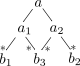
\includegraphics[width=0.195\linewidth]{../newman_3}
%   \caption{}
% \end{figure}

    Ponieważ \(b_1 \neq b_2\), to albo \(b_1 \neq b_3\), albo \(b_2 \neq b_3\).
    Możemy więc wybrać \(a'=a_1\) lub \(a'=a_2\). Kontynuując tę konstrukcję widzimy, że otrzymujemy nieskończoną redukcję, wbrew założeniu, że \(\to\) ma własność \(SN\).

    Zatem nie istnieją elementy wieloznaczne.\qed
\end{enumerate}
\end{minipage}
  \begin{minipage}{.25\textwidth}
    \begin{center}  
    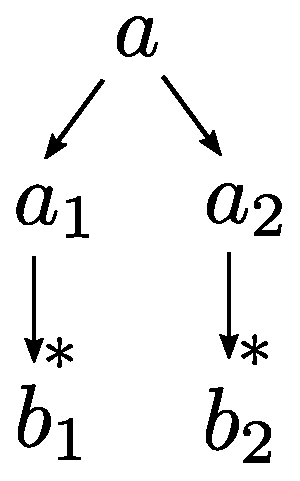
\includegraphics[width=0.41\linewidth]{../newman_1}
    \vspace{2em}

    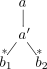
\includegraphics[width=0.41\linewidth]{../newman_2}
    \vspace{2em}

    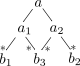
\includegraphics[width=0.71\linewidth]{../newman_3}
    \end{center}
  \end{minipage}
\end{dowod}
